\chapter{TikTok Analytics Exporter}
\label{sec:TikTok Analytics Exporter}

The TikTok Analytics Exporter is a Chrome extension that enables TikTok creators to generate structured backups of their own TikTok Studio analytics and optionally donate those files to the research team. The extension exports two categories of data: (1) per-video performance metrics over a user-selected date range, and (2) up to 365 days of daily follower history. Both are exported as Comma-Separated Value (CSV) files, saved directly onto the participants local disk.

\section{System Architecture}

\begin{figure}[h]
    \centering
    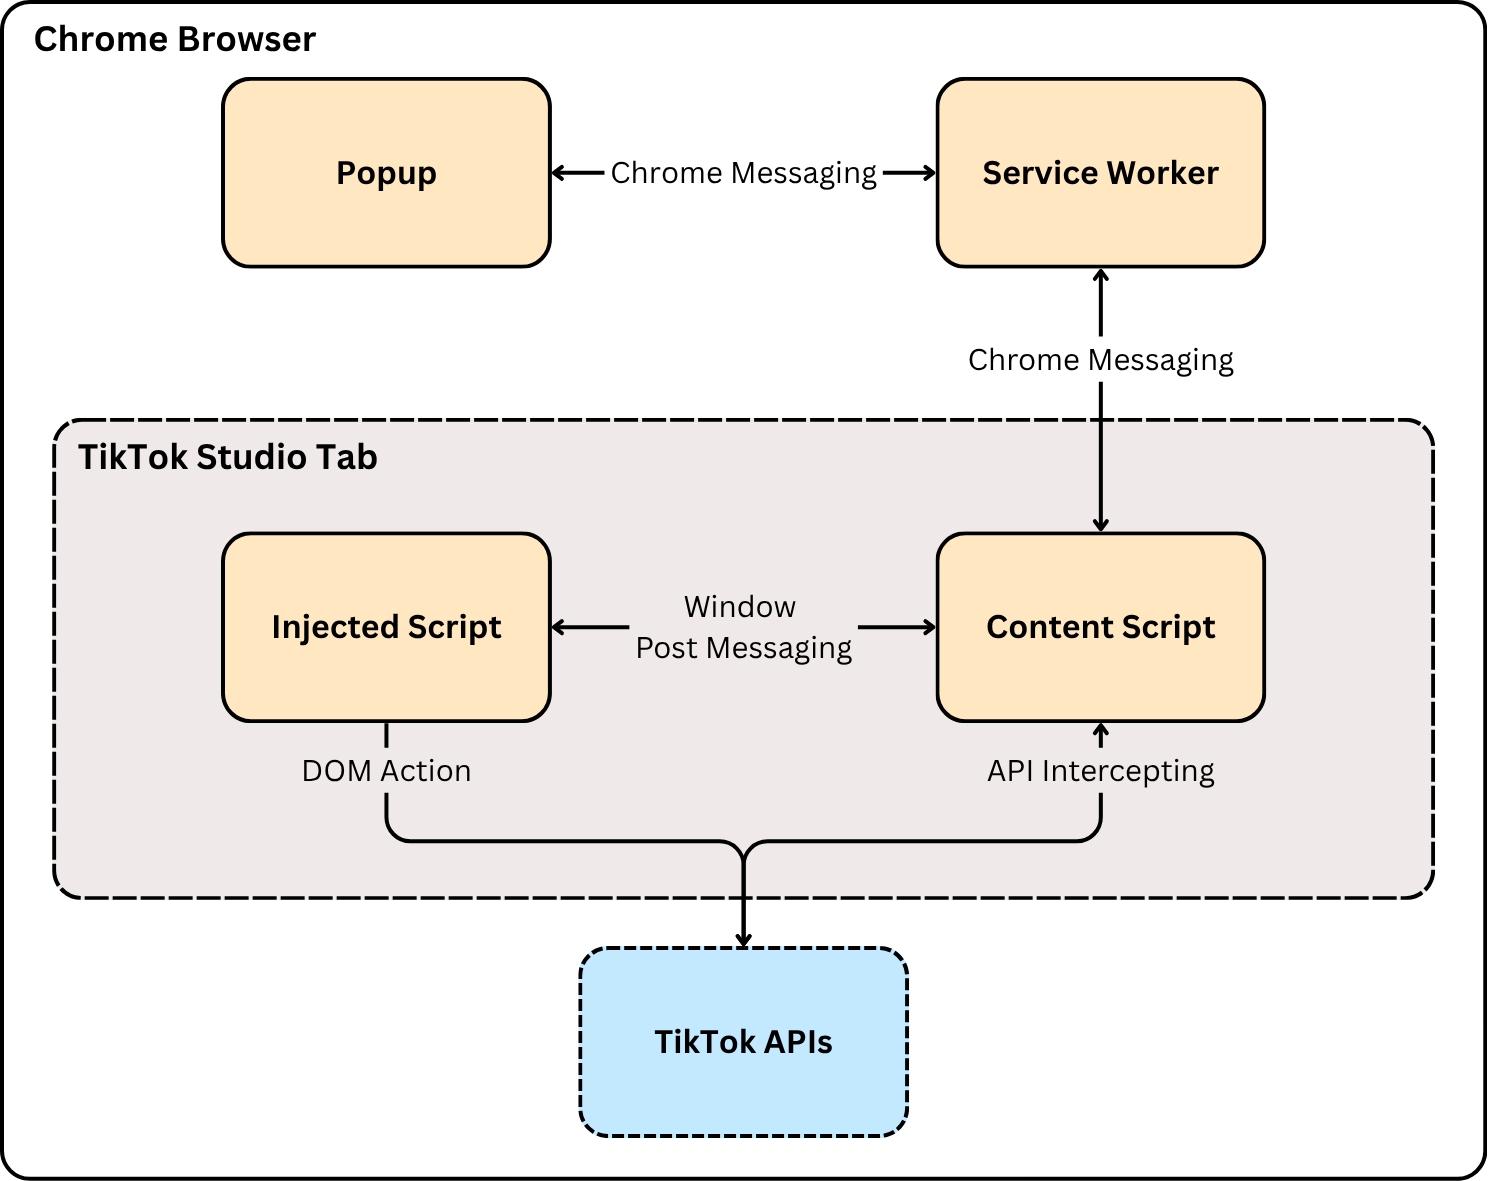
\includegraphics[width=1\linewidth]{figures/chap5/extension-architecture.png}
    \caption[TikTok Analytics Exporter Extension Architecture Overview]
    {Architecture of the extension across its four browser execution contexts (popup, service worker, content script, injected script), showing that data is captured into local session storage and only written to CSV on an explicit creator-initiated export.}
    \label{fig:extension-architecture}
\end{figure}

The extension operates entirely within the user's browser, utilizing a high-level architecture designed for simplicity and privacy. As the user navigates TikTok Studio, the browser communicates directly with the TikTok API to fetch analytics data. An overview of the extension's architecture is shown in Figure \ref{fig:extension-architecture}.

Instead of having a persistent background process, the extension passively intercepts this data and stores it temporarily in the browser's session storage. This in-browser session storage acts as the primary mechanism for maintaining state. When the user initiates an export, the extension compiles this locally stored data into a structured format without making any additional API requests, ensuring that the export process is entirely self-contained and relies only on the data already present on the user's machine.

\section{User Flow}

\subsection{Installation}
\label{sec:ext_installation}

Shown in Figure \ref{fig:extension-installation} is the step-by-step procedure for installing the extension. To install the extension, the user must be using a Chrome (or Chromium-based) browser and navigate to \texttt{chrome://extensions}. Then, enable Developer mode on the top-right part of the screen. After that, the user clicks on Load unpacked and selects the folder containing the extension. 

\begin{figure}[h]
    \centering
    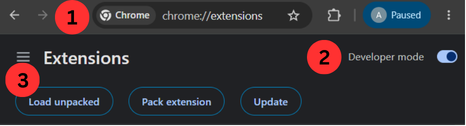
\includegraphics[width=1\linewidth]{figures/chap5/extension-install.png}
    \caption[Step-by-step procedure on installing the extension.]
    {Step-by-step installation of the extension in a Chrome or Chromium-based browser. Step 1: navigate to \texttt{chrome://extensions}. Step 2: toggle Developer Mode on. Step 3: click Load Unpacked and select the extension folder.}
    \label{fig:extension-installation}
\end{figure}

The user should see the TikTok Analytics Exporter in the list of their extensions, as shown in Figure \ref{fig:extension-installed}.

\begin{figure}[!h]
    \centering
    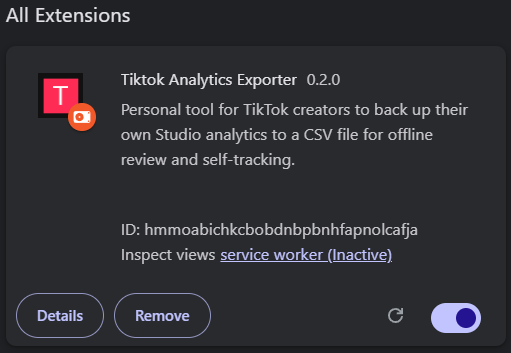
\includegraphics[width=0.8\linewidth]{figures/chap5/extension-installed.png}
    \caption[TikTok Analytics Exporter is installed.]
    {Confirmation that the extension is installed: the TikTok Analytics Exporter appears as an enabled entry in the \texttt{chrome://extensions} list.}
    \label{fig:extension-installed}
\end{figure}

\subsection{Video Analytics Export}
\label{sec:ext_video_export}

To export video analytics, the user should first navigate to TikTok Studio, then select Posts in the left navigation bar, as shown in Figure \ref{fig:tiktok-content}. Then, the user opens the extension popup, optionally selects a date range (with the default being the last 1 year), and clicks "Extract video stats," as shown in \ref{fig:ext-extract video stats}. The user is then presented with a summary of the extracted data and a prompt to save the results on their local computer as a CSV file, as shown in Figure \ref{fig:ext-video-done}.

\begin{figure}
    \centering
    \begin{subfigure}{0.35\textwidth}
        
\includegraphics[width=\textwidth]{chap5/tiktok-content.png}
        \caption{Step 1: Navigate to Posts. The creator opens TikTok Studio and clicks Posts in the left sidebar to display the video list.}
        \label{fig:tiktok-content}
    \end{subfigure}
    \hfill
    \begin{subfigure}{0.62\textwidth}
        
\includegraphics[width=\textwidth]{chap5/extension-video-export.png}
        \caption{Step 2: Extract video stats. The creator opens the extension popup, sets the desired date range, and clicks Extract Video Stats.}
        \label{fig:ext-extract video stats}
    \end{subfigure}
    
    \vspace{0.5cm}
    
    \begin{subfigure}{0.62\textwidth}
        
\includegraphics[width=\textwidth]{chap5/ext-video-done.png}
        \caption{Step 3: Save CSV. The extension displays a summary of the extracted videos and prompts the creator to save the results as a CSV file.}
        \label{fig:ext-video-done}
    \end{subfigure}

    \caption[Three-step video analytics export flow.]
    {The three-step video analytics export flow: navigate to TikTok Studio's Posts page, extract video stats via the extension popup, and save the resulting CSV to the local disk.}
    \label{fig:video-export-user-flow}
\end{figure}

\subsection{Follower History Export}
\label{sec:ext_follower_export}

\begin{figure}[!b]
    \centering
    \begin{subfigure}{0.8\textwidth}
        
\includegraphics[width=\textwidth]{chap5/tiktok-followers.png}
        \caption{Step 1: Navigate to Followers. The creator opens TikTok Studio, clicks Analytics in the left sidebar, then selects the Followers tab.}
        \label{fig:tiktok-followers}
    \end{subfigure}

    \vspace{0.5cm}

    \begin{subfigure}{0.48\textwidth}
        
\includegraphics[width=\textwidth]{chap5/ext-extract-followers.png}
        \caption{Step 2: Extract follower history. The creator opens the extension popup and clicks Extract Follower History to begin retrieval.}
        \label{fig:extract-followers}
    \end{subfigure}
    \hfill
    \begin{subfigure}{0.48\textwidth}
        
\includegraphics[width=\textwidth]{chap5/ext-follower-save.png}
        \caption{Step 3: Save CSV. The extension displays the retrieved follower data and prompts the creator to save up to 365 days of daily follower history as a CSV file.}
        \label{fig:save-followers}
    \end{subfigure}

    \caption[Three-step follower history export flow.]
    {The three-step follower history export flow: navigate to TikTok Studio's Followers analytics page, extract follower history via the extension popup, and save the resulting CSV to the local disk.}
    \label{fig:video-export-user-flow}
\end{figure}

To export follower history, the user navigates to the TikTok Studio analytics page, click on Analytics in the left sidebar, then click Followers at the top, shown in Figure \ref{fig:tiktok-followers}. Then, the user can click on "Extract follower history" in the extension, shown in Figure \ref{fig:extract-followers}. The extension retrieves the follower data automatically and, upon completion, prompts the user to save the results as a CSV file containing up to the last 365 days of follower history, shown in Figure \ref{fig:save-followers}.

\subsection{Completion}

When both exports are complete, the extension displays a banner confirming that both files can be saved locally, as seen in Figure \ref{fig:both-ready}. The user may then share the CSV files with the research team through the data collection site, TokDrop.

\begin{figure}[h]
    \centering
    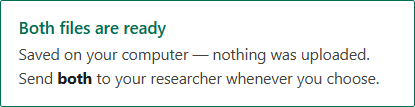
\includegraphics[width=0.8\linewidth]{figures/chap5/ext-both-ready.png}
    \caption[Completion state of the extension]
    {Completion state of the extension. A banner confirms that both the video-analytics CSV and the follower-history CSV have been generated and can be saved locally.}
    \label{fig:both-ready}
\end{figure}

\section{Data Derivation and Extraction Schema}

\subsection{Video Metadata Collection}

Video metadata such as IDs, timestamps, captions, and basic engagement counts are collected passively during the scroll phase of the video export workflow. The extension intercepts these responses and extracts structured records from them.

Because TikTok has been observed to use different property names and nesting structures across its various front-end surfaces and API versions, the extraction algorithm employs a multi-strategy approach. It first attempts to locate the video array at twelve known property paths (such as json.item\_list, json.itemList, json.aweme\_list, and json.data.item\_list). If none of these yields a non-empty array, it falls back to a bounded breadth-first search of the JSON tree looking for any array whose first element satisfies a heuristic check for characteristic video item fields (aweme\_id, create\_time, statistics). Field names are then normalized across API versions: for instance, both create\_time and createTime are accepted, as are desc, caption, and text for the video caption field. The resulting records are stored in an object map keyed by aweme\_id, providing O(1) deduplication when responses from overlapping pages arrive.

\subsection{Insight Data Retrieval}

Detailed per-video analytics like watch times and retention curves are not available in video list responses and must be retrieved separately from TikTok's insight API. When the user browser TikTok studio, the extension obtains a reusable template. One insight API call is issued per video. The response parser uses a depth-first search algorithm with an explicit stack to avoid recursion limits to locate each target metric within TikTok's variably nested response structure.

\subsection{Follower History Retrieval}

The follower history export issues a single API call requesting three metric types simultaneously: the daily cumulative follower count, the current follower count which used as an anchor, and the daily net follower change. The response is trimmed to the last 365 days in the parser.

\subsection{Output Schema}

The extension produces two CSV files with their column structures described in Tables \ref{tab:video_performance_csv} and \ref{tab:follower_history_csv}.

\begin{table}[H]
\centering
\begin{tabular}{p{0.33\textwidth} p{0.60\textwidth}}
\toprule
\textbf{Field} & \textbf{Description} \\
\midrule
\texttt{video\_id} & Unique identifier of the video. \\
\texttt{post\_date} & Date the video was published. \\
\texttt{post\_time} & Time the video was published. \\
\texttt{caption} & Caption or text accompanying the video. \\
\texttt{duration\_ms} & Duration of the video in milliseconds. \\
\texttt{comments} & Total number of comments received. \\
\texttt{shares} & Total number of shares. \\
\texttt{ECR} & Engagement rate (Engagement Continuation Rate). \\
\texttt{avg\_watch\_time\_s} & Average watch time in seconds. \\
\texttt{NAWP} & Normalized Average Watch Percentage. \\
\texttt{watched\_full\_pct} & Percentage of viewers who watched the entire video. \\
\texttt{traffic\_foryou\_pct} & Percentage of traffic originating from the For You feed. \\
\texttt{traffic\_follow\_pct} & Percentage of traffic originating from followers. \\
\texttt{traffic\_profile\_pct} & Percentage of traffic originating from profile visits. \\
\texttt{traffic\_search\_pct} & Percentage of traffic originating from search. \\
\texttt{new\_followers} & Number of new followers gained from the video. \\
\texttt{data\_quality} & Indicator of the completeness or validity of the exported data. \\
\bottomrule
\end{tabular}
\caption{Video Performance CSV fields and corresponding descriptions}
\label{tab:video_performance_csv}
\end{table}

\begin{table}[H]
\centering
\begin{tabular}{p{0.33\textwidth} p{0.60\textwidth}}
\toprule
\textbf{Field} & \textbf{Description} \\
\midrule
\texttt{date} & Date of the recorded follower statistics. \\
\texttt{follower\_count} & Total number of followers on the recorded date. \\
\texttt{daily\_net} & Net change in followers for the recorded date. \\
\texttt{creator\_handle} & TikTok username of the creator. \\
\texttt{creator\_uid} & Unique identifier of the creator. \\
\texttt{data\_quality} & Indicator of the completeness or validity of the exported data. \\
\bottomrule
\end{tabular}
\caption{Follower History CSV fields and corresponding descriptions}
\label{tab:follower_history_csv}
\end{table}

\subsection{Metric Derivation}

\subsubsection{Engagement Continuation Rate (ECR)}

ECR is the probability that the viewer will continue watching the video after the first 5 seconds. This is extracted from TikTok's video\_retention\_rate\_realtime metrics, which provides a time-indexed retention curve for each video. The extension reads the retention value at the 5,000 millisecond mark.

\subsubsection{Normalized Average Watch Percentage (NAWP)}

NAWP is a normalized measure of viewer retention over a whole video. This is computed within the parser as
\begin{equation}
    \text{NAWP} = \frac{\text{avg\_watch\_time\_s}}{\text{duration\_ms} / 1000}
\end{equation}
where $\text{avg\_watch\_time\_s}$ is taken from the insight response and $\text{duration\_ms}$ comes from the video metadata.

This normalization expresses the average watch time as a fraction of the total video duration, producing a value in the range $[0,1]$. This makes it comparable across videos of different lengths.
